\chapter{Background}

\section{CSMA and TDMA} \label{A.1}

\begin{figure}[h!]
\centering
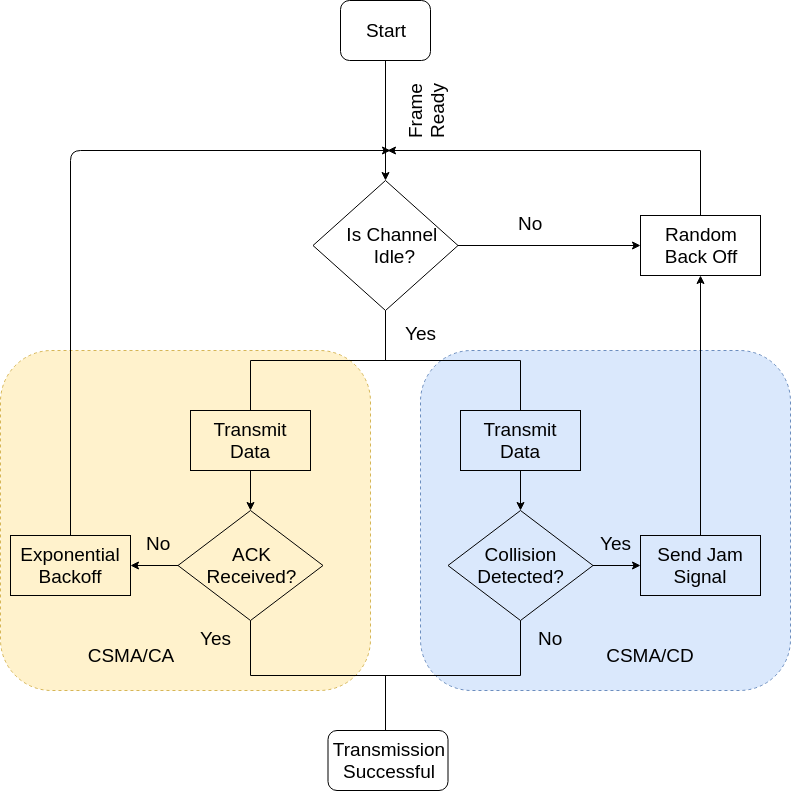
\includegraphics[width=0.9\textwidth]{Figure/CSMA.png}
\caption{CSMA flow graph.}
\label{Csma_flow}
\end{figure}

\ac{csma} is a \ac{L2} protocol in the OSI Model. 
%It is a method for handling multiple access of a shared medium.
It mainly comes in two varieties: \ac{CSMA/CD}  and \ac{CSMA/CA}.
The flow graphs of both are shown in Figure \ref{Csma_flow}.
In the older \ac{CSMA/CD}, the nodes checks the idleness of the channel after the frame is ready.
If idle it starts transmission.
During transmission, it monitors the medium for collision.
If collision is detected, it employs a collision recovery process, where it sends a jam signal to signal other nodes that a collision has occurred.
Then it waits for a  random delay and starts transmission again.\\

\ac{CSMA/CA} tries to avoid collision, it starts off similar to \ac{CSMA/CD} where it senses to check when the channel is idle.
If found idle, it starts transmission.
It is difficult for wireless nodes to detect collisions simultaneously during transmission.
Therefore, it relies on an \ac{ack} message from the receiving node to check if the data packet was received.
If \ac{ack} is not received, the node assumes a collision has occurred and  uses exponential back-off to determine when the next time to re initiate transmission.\\


\ac{tdma} is also a \ac{L2} protocol, where a coordinator schedules medium access to the nodes in a periodic manner.
Communication happens in time-slots.
Each node in the network is given exclusive access to transmit during its time slot.
The coordinator generates beacon signals periodically to maintain relative time synchronization. On receiving the beacons, the nodes adjust their transmit clocks so that they have the correct estimate of their time-slots.

\section{GNU Radio} \label{A.2}

\subsection{GNU Radio Block Types}
\begin{table}[h!]
\centering
\begin{tabular}{|c|c|c|}
\hline
Number of input elements & Number of output elements & Name\\
\hline
N & 0 & Sink Block\\
0 & N & Source Block\\
N & 1 & Interpolation block\\
1 & N & Decimation block\\
M & N & General Block\\
\hline
\end{tabular}
\caption{GNU Radio Block Types}
\label{block_type}
\end{table} 

The relationship of input and output elements defines the type of the GNU Radio processing block as shown in Table \ref{block_type}.
The type of block indicates the scheduler on how the block processes information.
There are two types of blocks: \textit{Synchronous block} and \textit{block}.
For synchronous blocks, there is a rational relationship between the input and output elements.
The sink, source, interpolation block and decimation block in Table \ref{block_type} are synchronous blocks.
The key difference between different block types is in how the scheduler handles the input and output buffers of each block.
For the synchronous blocks, the scheduler implicitly handles the input and output pointers to the buffers.
For general blocks, the \textit{work} function needs to explicitly pass the information on how many elements it consumed and produced.\\

\subsection {GNU Radio Interfaces}
Since in GNU Radio flow graph, data is passed from one node to another, the method of passing the data among different blocks needs to be defined.
This method is defined in the block interfaces.
Stream Interfaces are intended to stream large amounts of data between blocks with variable processing rates.
They use large buffers to pass the data from one node to another.
Stream interfaces work well for samples, bits etc. but they are not the right method to pass metadata, control information or bursts of data between blocks as it involves significant overhead.\\

GNU Radio recently added the message passing interface for handling asynchronous message passing.
GNU Radio also supports stream tags for handling metadata as it is closely associated with the stream data samples.
Stream tags are attached with stream data samples and provide additional information associated with the sample.
It can be used both for passing control flags as well as metadata information like the \ac{PDU} size, timing information etc.
These stream tags are propagated to the next blocks and is updated by the data rate changes.
For example, if the block takes it 2 samples as input and produces 4 samples as output, its data rate is 2.
In this case, if the input stream had a stream tag at position $x$ then the the location in the output stream would be $2x$. \\

\section{LMS7002M} \label{A.3}

\begin{figure}[h!]
\centering
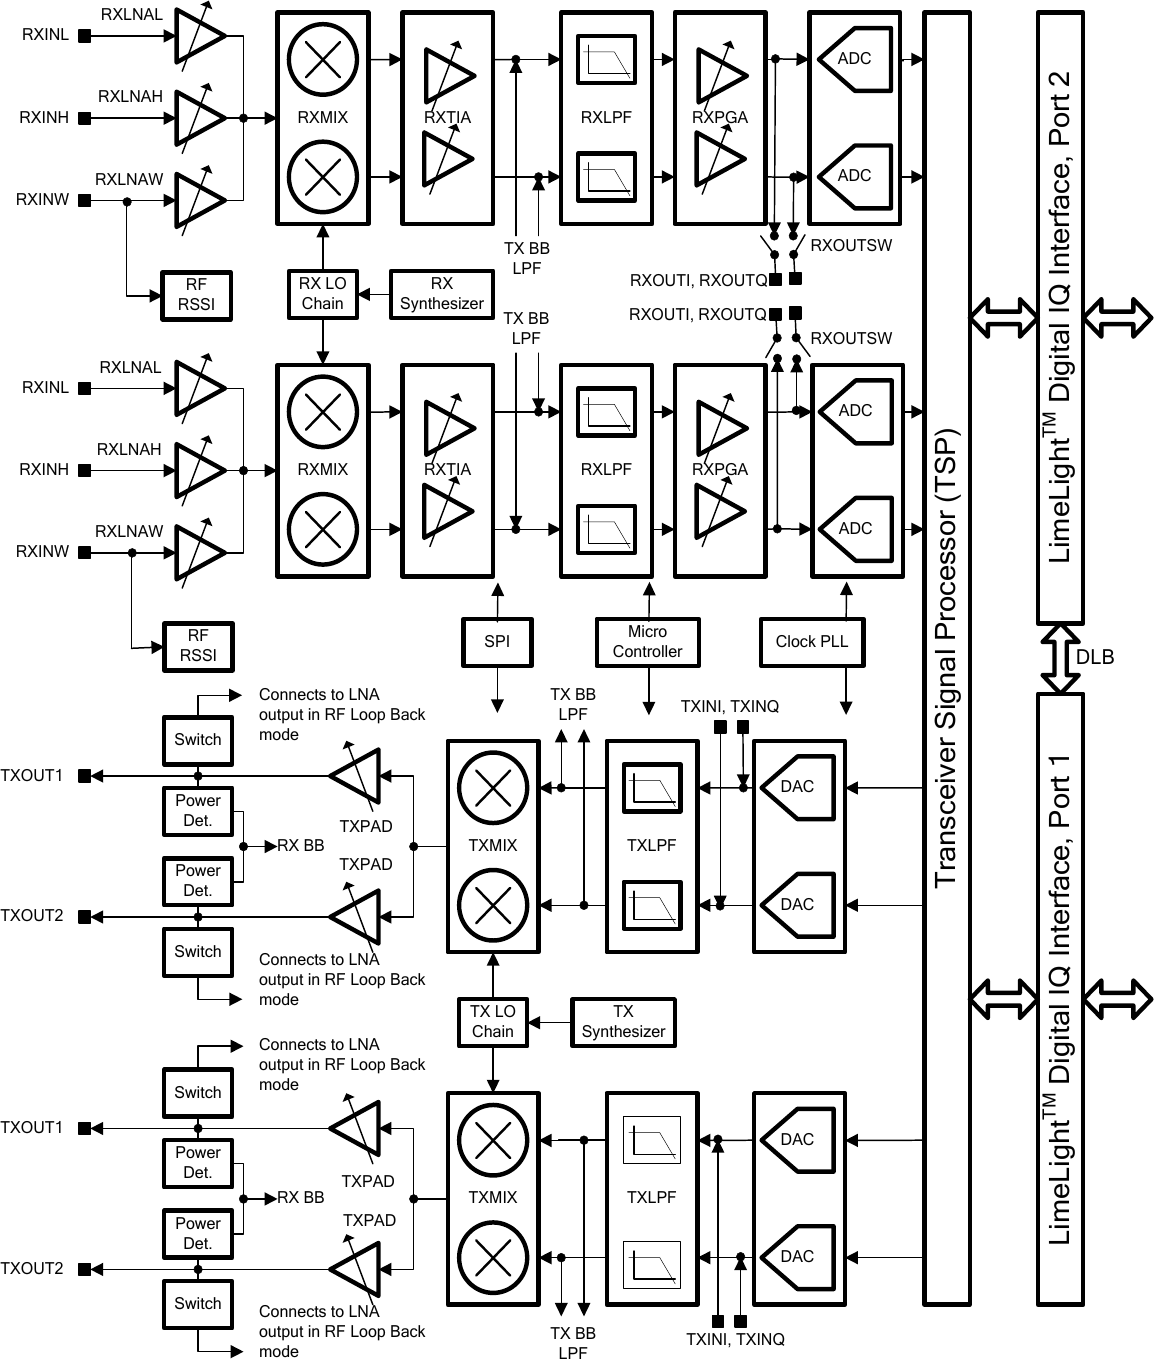
\includegraphics[width=0.9\textwidth]{Figure/Lms7002m-block-diagram.png}
\caption{Block Diagram of LMS7002M.}
\label{lms7002m}
\end{figure}

LMS7002M offers full duplex communication link on both the TX and RX chains.
Each of the RX chains has three separate \ac{RF} ports tuned for narrow band low frequency, narrow band high frequency and wide band operations.
Similarly, the TX Chains are connected two separate \ac{RF} ports tuned for high frequency and low frequency operations.
This separation is done for better impedance matching at the boundary of the antennas.\\

Figure \ref{lms7002m} shows the functional block diagram for a LMS7002M \ac{FPRF}.
Since, both the RX and TX paths are identical, the report concentrates on only one RX path.
The output from the \ac{RF} RX ports are fed into the \ac{LNA} inorder to minimize injecting too much noise at the beginning of the chain.
The receiver follows the architecture shown in Figure \ref{rf_receiver}, with a RX mixer, followed by filter and a \ac{PGA} combined in a Zero-IF architecture.
The RX \ac{PGA} outputs the analog baseband signal.\\

LMS7002M uses a fractional N-\ac{PLL} architecture for the local oscillator frequency synthesis.
\ac{PLL} is used extensively in \ac{RF} circuits for making sure the generated local oscillator signal and the reference signal have the same phase and frequency.
PLLs are essentially negative feedback systems, so when the input signal differs a lot from the output signal, the control logic tries to lower the error (\textit{input-output)}.\\

Integer N- \ac{PLL} architectures are used to generate high frequency signals from low frequency reference clocks, by using a frequency divider in the negative loopback path.
The frequency divider is basically a counter, that outputs every "N" (division factor of the loop) clock cycles of the output signal.
But since the output signal frequency will be multiples of the reference clock, the output signal resolution is determined by the  reference clock.\\

So to have a high frequency as well as a high resolution, the divider counter should be very large in size.
To counter the problem, fractional N-{PLL} architectures were designed where the output signal frequency can also be a fractional multiple of the input signal frequency.
This helps in increasing the frequency resolution without the need for a large divisor counter.
The input and output frequency relationship for a fractional  N-\ac{PLL} can be summarized by: $f_{out}=f_{ref}(N+k/M)$, where N is the integer divider factor, k is the fractional divider factor and $1/M$ gives the output frequency resolution.
Both the integer and fractional divider factor are determined by the size of the counters used.
In case of LimeSDR, the reference signal fed to the PLL varies from to 10 to 52 MHz.
The output signal can vary from 30 to 3800 MHz, with a frequency resolution of 24.8 Hz.\\

Once the \ac{RF} demodulation is completed by the analog processing chain, the analog signal is sent to the data converters and converted to digital data samples.
The sampling rate for the data conversion is determined by the required \ac{RF} channel bandwidth.
The digital samples are sent to the \ac{TSP} for further processing.\\

The \ac{TSP} uses advanced signal processing algorithms like IQ DC offset correction, IQ phase correction for correcting the received samples.
An interpolation and decimation filter is added to the \ac{TSP} for the TX and RX chains respectively.
These filters are implemented with a chain of five fixed co-efficient half band \ac{FIR} filters, which allows interpolation and decimation factors of 1,2,4,8,16.
Interpolation and Decimation allows the baseband to run at a lower data rate while still running the data converters at higher sampling rates, enabling the quantization noise to be spread over larger frequency range.
Automatic Gain Control is also implemented by the the \ac{TSP}.\\

\section{USBMon}
The details about the USBMon IO Traces for the text and raw binary interfaces is presented here.

\subsubsection{Text Data Format}
\begin{table}[h!]
\centering
\begin{tabular}{|c|c|c|c|c|}
\hline
URB Tag & Timestamp & Event Type & Address & URB Status\\
\hline
ffff8fbdbbae4000 & 2942307806 & S & Bo:3:008:15 & -115\\ 
\hline
\end{tabular}
\begin{tabular}{|c|c|c|}
\hline
Data Length & Data Tag & Data\\
\hline
64 & = & 21000100 00000000 002a0484 00000000 000000\\
\hline
\end{tabular}
\caption{Text USB Trace Example.}
\end{table}

\begin{itemize}
\item {\textbf{URB Tag:} URB Identification number, it is usually the in kernel adress of the URB structure.}
\item{\textbf{Timestamp:} The timestamp for the URB event at the HCD in microseconds. It is measured by the usbmon main utility using \textit{gettimeofday()} function of \textit{time.h}.}
\item{\textbf{Event Type:} It specifies the event type of the HCD event. S - Submission C -Complete E - submission error.}
\item{\textbf{Address: } It consists of four fields separated by colons. The URB type and direction, bus number, device number, endpoint number. The URB type and direction specifies the type of USB transfer(can be both synchronous and asynchronous).\\
\begin{table}[h!]
\centering
\begin{tabular}{|c|c|c|}
\hline
Bi & Bo & Bulk Input and Output.\\
Ci & Co & Control Input and Output.\\
Ii & Io & Interrupt Input and Output.\\
Zi & Zo & Isochronous Input and Output.\\
\hline
\end{tabular}
\caption{URB Type and Direction.}
\end{table}\\
The USB device transfers data through a pipe to a memory buffer on the host and endpoint on the device. The type of data transfer depends on the endpoint and the requirements of the function. The transfer types are as follows\cite{_usb_data_transfer}:

\begin{itemize}
\item{\textbf{Control Transfers:} It is mainly used for configuration, command and status operations.}
\item{\textbf{Bulk Transfers:} Bulk Transfer are used for bulky,non-periodic non time-sensitive burst transmissions.}
\item{\textbf{Interrupt Transfers:} It is used for mainly sending small amounts of data infrequently or asynchronously.}
\item{\textbf{Isochronous Transfers:} Isochronous transfers are mainly used for periodic, continuous streams of time sensitive data.} 
\end{itemize}
%USB endpoint as explained by \cite{_usb_endpoint} , refers to the buffers on the USB device. The host computer irrespective of the host operating system can communicate by reading and writing to these buffers. They can be data endpoints and control endpoints.Data endpoints are used for transferring data whereas the control endpoint is used for configuration and device specific control.
}

\item{\textbf{Data Length:} For urb\_submit it gives the requested data length and for callbacks it is the actual data length.}

\item{\textbf{Data tag:} If this field is '=' then data words are present.}

\item{\textbf{Data:} The data words contains in the USB transfer packet.}
\end{itemize}

\subsubsection{Raw Binary}
The overall data format is same as the text data, the data is available in raw binary by accessing character devices at /dev/usbmonX. The data can be read by using \textit{read} with \textit{ioctl} or by mapping the buffer using \textit{mmap}. The usbmon events are buffered in the following format:

\begingroup
\centering\scriptsize\begin{lstlisting}
struct usbmon_packet {
	u64 id;			/*  0: URB ID - from submission to callback */
	unsigned char type;	/*  8: Same as text; extensible. */
	unsigned char xfer_type; /*    ISO (0), Intr, Control, Bulk (3) */
	unsigned char epnum;	/*     Endpoint number and transfer direction */
	unsigned char devnum;	/*     Device address */
	u16 busnum;		/* 12: Bus number */
	char flag_setup;	/* 14: Same as text */
	char flag_data;		/* 15: Same as text; Binary zero is OK. */
	s64 ts_sec;		/* 16: gettimeofday */
	s32 ts_usec;		/* 24: gettimeofday */
	int status;		/* 28: */
	unsigned int length;	/* 32: Length of data (submitted or actual) */
	unsigned int len_cap;	/* 36: Delivered length */
	union {			/* 40: */
		unsigned char setup[SETUP_LEN];	/* Only for Control S-type */
		struct iso_rec {		/* Only for ISO */
			int error_count;
			int numdesc;
		} iso;
	} s;
	int interval;		/* 48: Only for Interrupt and ISO */
	int start_frame;	/* 52: For ISO */
	unsigned int xfer_flags; /* 56: copy of URB's transfer_flags */
	unsigned int ndesc;	/* 60: Actual number of ISO descriptors */
};	
\end{lstlisting}
\endgroup
